\documentclass[a4paper, oneside, 11pt]{book} % we are not printing this like a book
\usepackage[hmargin=2cm,vmargin=2.5cm,bindingoffset=0.5cm]{geometry}
\usepackage[colorlinks=true]{hyperref}
\usepackage{bookmark}
\usepackage{graphicx}
\usepackage{subfiles}
\usepackage{fancyhdr}
\usepackage{fontspec}
\usepackage{titlesec}
\usepackage{minted}
\usepackage{longtable}
\usepackage{float}
\usepackage{tabularx}
\usepackage[table]{xcolor}
\usepackage{array}
\usepackage{csquotes}
\usepackage{plex-serif}

\newfontfamily\mono{Iosevka Fixed Extended} % For monospace
\setmonofont{Iosevka Fixed Extended}
%\setmainfont{IBM Plex Serif}

\definecolor{lightlightgray}{rgb}{0.95, 0.95, 0.95}

\usepackage{cellspace}
\setlength\cellspacetoplimit{10pt} % Minimum space above cell content
\setlength\cellspacebottomlimit{10pt} % Minimum space below cell content

% italic captions
\usepackage[format=plain,
            labelfont=it,
            textfont=it]{caption}

% nicer footnotes
\usepackage[splitrule]{footmisc}

% font spacing
\setlength{\spaceskip}{0.55em plus 0.15em minus 0.15em}

% image paths
\graphicspath{{./images/}}

% paragraph spacing
\setlength{\parskip}{1em}
% no indenting paragraphs (its 2025)
\setlength{\parindent}{0pt}

% nicer paragraph headings
\usepackage{titlesec}
\titleformat{\paragraph}
  {\normalfont\bfseries}
  {}
  {0pt}
  {} 
\titleformat{\subparagraph}
  {\normalfont\bfseries}
  {}
  {0pt}
  {}

% page styling
\pagestyle{fancy}
\setlength{\headheight}{15pt}
\fancyhf{}
\fancyhead[L]{\small \textbf{The IGCSE Computer Science Revision Guide}}
\fancyhead[R]{\nouppercase{\leftmark}}
\fancyfoot[C]{\thepage}

\setlength{\arrayrulewidth}{0.3pt}
\renewcommand{\arraystretch}{1.3}

\setminted{
    bgcolor=lightlightgray,
    linenos=true,
    tabsize=4
}

\definecolor{red}{HTML}{d61111}
\definecolor{blue}{HTML}{1356b7}
\definecolor{green}{HTML}{22b625}
\definecolor{yellow}{HTML}{ffb206}

\definecolor{linkblue}{HTML}{206ac9}

\hypersetup{
    colorlinks=true,
    linkcolor=linkblue,
    citecolor=linkblue,
    filecolor=linkblue,
    urlcolor=linkblue
}

% info
\title{The IGCSE Computer Science (Theory) Revision Guide}

\author{\textbf{Eason Qin} (eason@ezntek.com),\\\textbf{Siddharth Harish} (sid.falcon9@gmail.com),\\\textbf{Karthik Sankar} (karthik@hackclub.com),\\and \textbf{Ved Jaggi} (ved@vedjaggi.com)}
\date{May 13th, 2025\\\emph{Fifth Revision}}

% da benin..beningi...benigi..da biningin™ 
\begin{document}

% Title Page

\newgeometry{margin=0pt}
\clearpage
\thispagestyle{empty}
\noindent
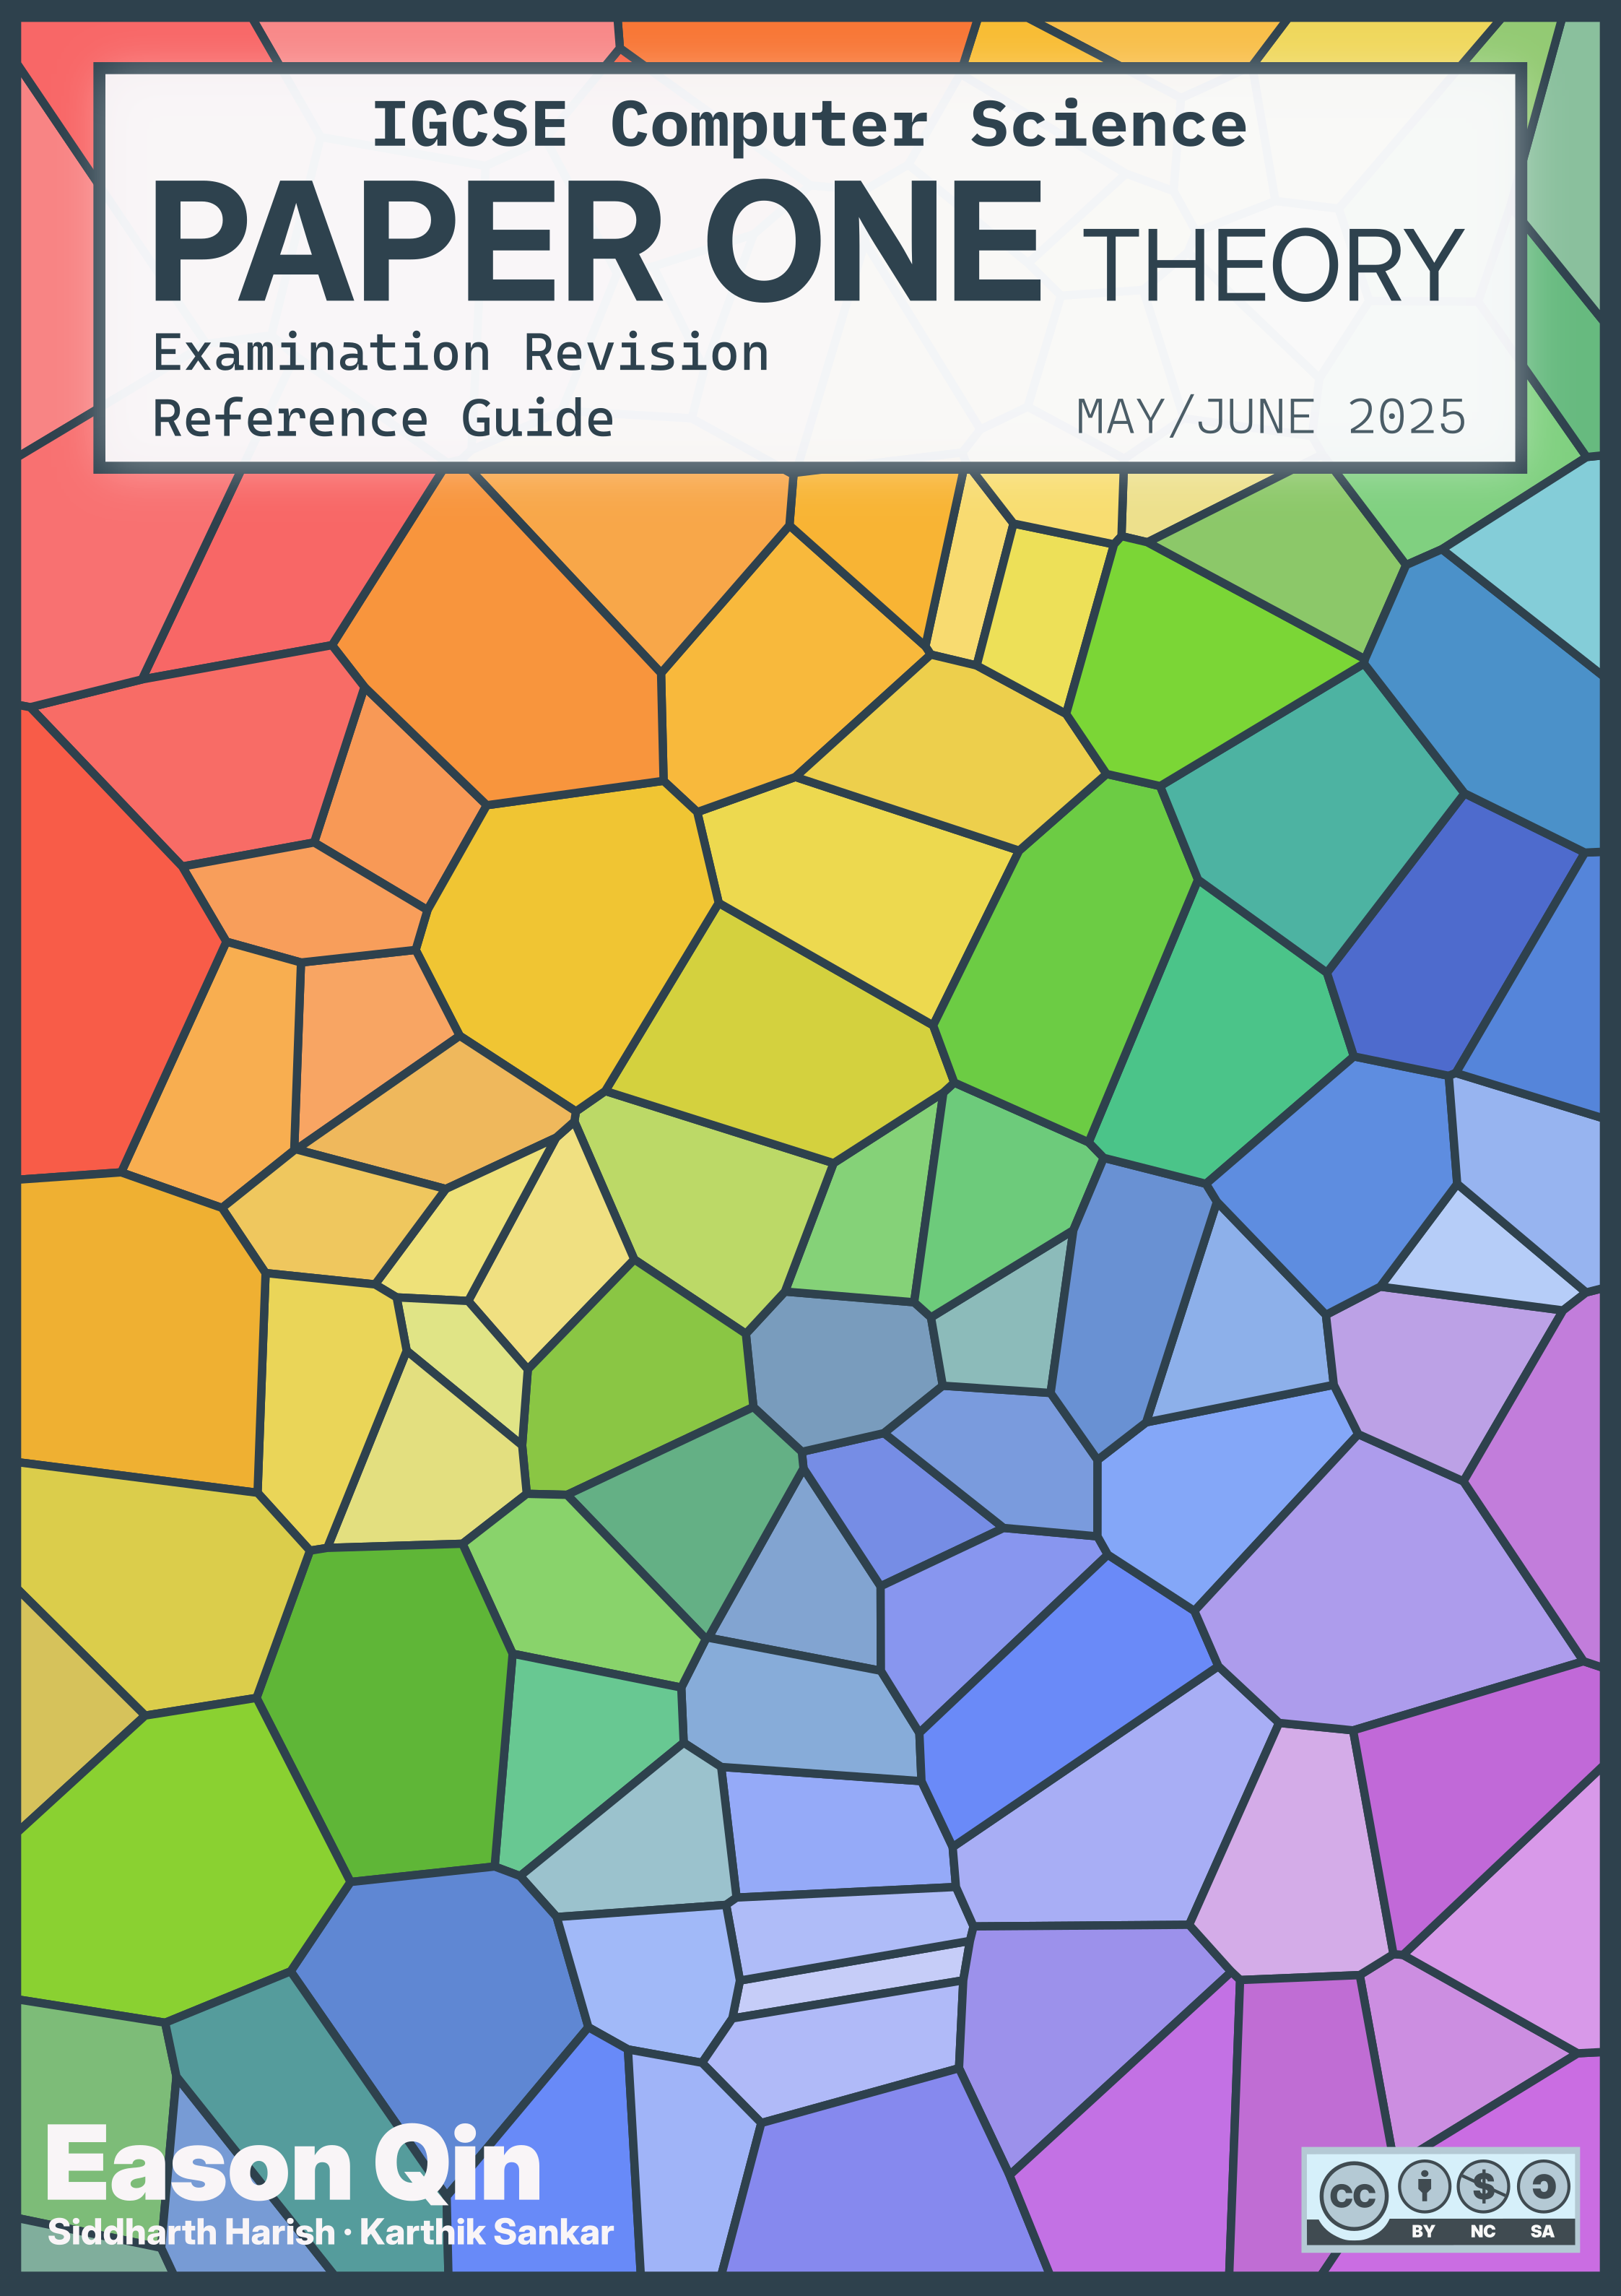
\includegraphics[width=\paperwidth,height=\paperheight,keepaspectratio=false]{cover.png}
\clearpage
\restoregeometry

% the inner title page
\maketitle
% TOC
\label{table-of-contents}
\tableofcontents

\chapter*{Introduction}
\addcontentsline{toc}{chapter}{Introduction}
\markboth{Introduction}{Introduction} % ew
\label{introduction}
\subfile{chapters/introduction}

\chapter{Data Representation}
\subfile{chapters/1_data_representation}

\chapter{Data Transmission}
\subfile{chapters/2_data_transmission}

\chapter{Hardware}
\subfile{chapters/3_hardware}

\chapter{Software}
\subfile{chapters/4_software}

\chapter{The Internet and Its Uses}
\subfile{chapters/5_the_internet_and_its_uses.tex}

\chapter{Emerging Technologies}
\subfile{chapters/6_emerging_technologies}

\end{document}
